\section{\wasm}
\label{sota:wasm}

\todo{Intro}

\subsection*{Overview}

% Javascript was first, and then more attempts.
Over the past decades, JavaScript has been used in the majority of the browsers vendors to allow client-side scripting. However, due to the complexity of the language and to gain in performance, several approaches appeared to introduce different languages.  For example, Java applets were introduced on web pages at \todo{XXX}, Adobe added ActionScript later on \todo{XXX}, Microsoft made an attempt with ActiveX \todo{XXX}. All these attempts failed, most of them due to security issues and lack of consensus on the community. 

% asm.js and the demonstration of bad language patterns
In 2014, Emscripten introduced a strict subset of JavaScript, asm.js, to allow low level code such as C to be compiled to JavaScript \todo{GG}. Asm.js was first implemented as an LLVM backend. This approach came with the benefits of having all the ahead-of-time optimizations from LLVM, gaining in twice the performance on browser clients \citationneeded compared to standard JavaScript code. The main reason why asm.js was faster, is that it limits the language features to those that can be optimized in the LLVM pipeline or those that can be directly translated from the source code. Besides, it removes the majority of the dynamic characteristics of the language, limiting it to numerical types, top-level functions, and one large array in the memory directly accessed as raw data. For example, C code won't be compiled to asm.js with nested functions. Since asm.js is a subset of JavaScript it was compatible with all engines. Asm.js demonstrated that client-code could be improved with the right language design and standarization.

% Limitations of asm.js and the birth of Wasm
The work of Van Es \etal \cite{EsAsm.js} proposed to shrink JavaScript to asm.js in a source-to-source strategy, closing the cycle and extending the fact that asm.js was mainly a compilation target for C/C++ code. Despite their result was encouraging, JavaScript faces several limitations related to the intrinsics of the language. For example, any JavaScript engine requires the parsing and the recompilation of the JavaScript code creating overhead \todo{Cryptic}. We, as many in the community consider asm.js the precursor of \wasm. The \wasm (Wasm) language was first publicly announced in 2015. \wasm is a binary instruction format for a stack-based virtual machine and was officially stated by the work of Haas \etal \cite{Haas_2017} in 2017. The announcement of \wasm marked the first step of standarizing bytecode in the web environment. Wasm is designed to be fast, portable, self-contained and secure, and it outperforms asm.js \citationneeded.

Since then, \wasm adoption has an exponential growth, companies like Adobe recently announced a full online version of Photoshop \citationneeded. Moreover, game companies moved their development from JavaScript to Wasm \citationneeded and stack technologies such as Microsoft implement their virtual machines in Wasm \citationneeded.

%\todo{Benchmarks}

\subsection*{From source to Wasm}

All \wasm programs are compiled ahead of time from source languages. LLVM includes Wasm as a target since version 8, supporting a broad range of frontend languages such as C/C++. The resulting binary, works similarly to a shared library, it includes instruction codes, symbols and exported functions. In \autoref{diagrams:sota:wasm}, we illustrate the workflow of the creation of Wasm binaries and their lifecycle. The process starts by compiling the source code program to Wasm (Step \step{1}). To the best of our knowledge, the best survey Wasm is presented in the Awesome Wasm (\url{https://github.com/mbasso/awesome-wasm}) repo. It is a cumulative GitHub repo which includes references to articles, papers, books, demos, compilers and engines. 

The step \step{2} includes the composition of the glue code to Wasm as JavaScript code. This code will include the harness that the Wasm binary needs. For example, by design, Wasm cannot access the DOM of the page as JavaScript code does and if need it, the functions to interact with the DOM are imported in the Wasm binary during its call. The glue JavaScript code can be manually written, however, compilers like Emscripten, Rust and Binaryen can generate it automatically.

Finally, the third step (Step \step{3}), includes the compilation of the client-side code. Most of the browser engines compile either the Wasm code or JavaScript to machine code. In the case of JavaScript this process involves JIT and hot code replacement during runtime. For Wasm, this process is almost direct, in the case of V8, only two compilation processes are required, a baseline compilation, meant to make the coming binary available as soon as possible and a final one, that makes some lane optimizations. This analysis was validated by conversations with the V8 develop team and by one experimental study in our contributions.  

\begin{figure}[h]
    \centering
    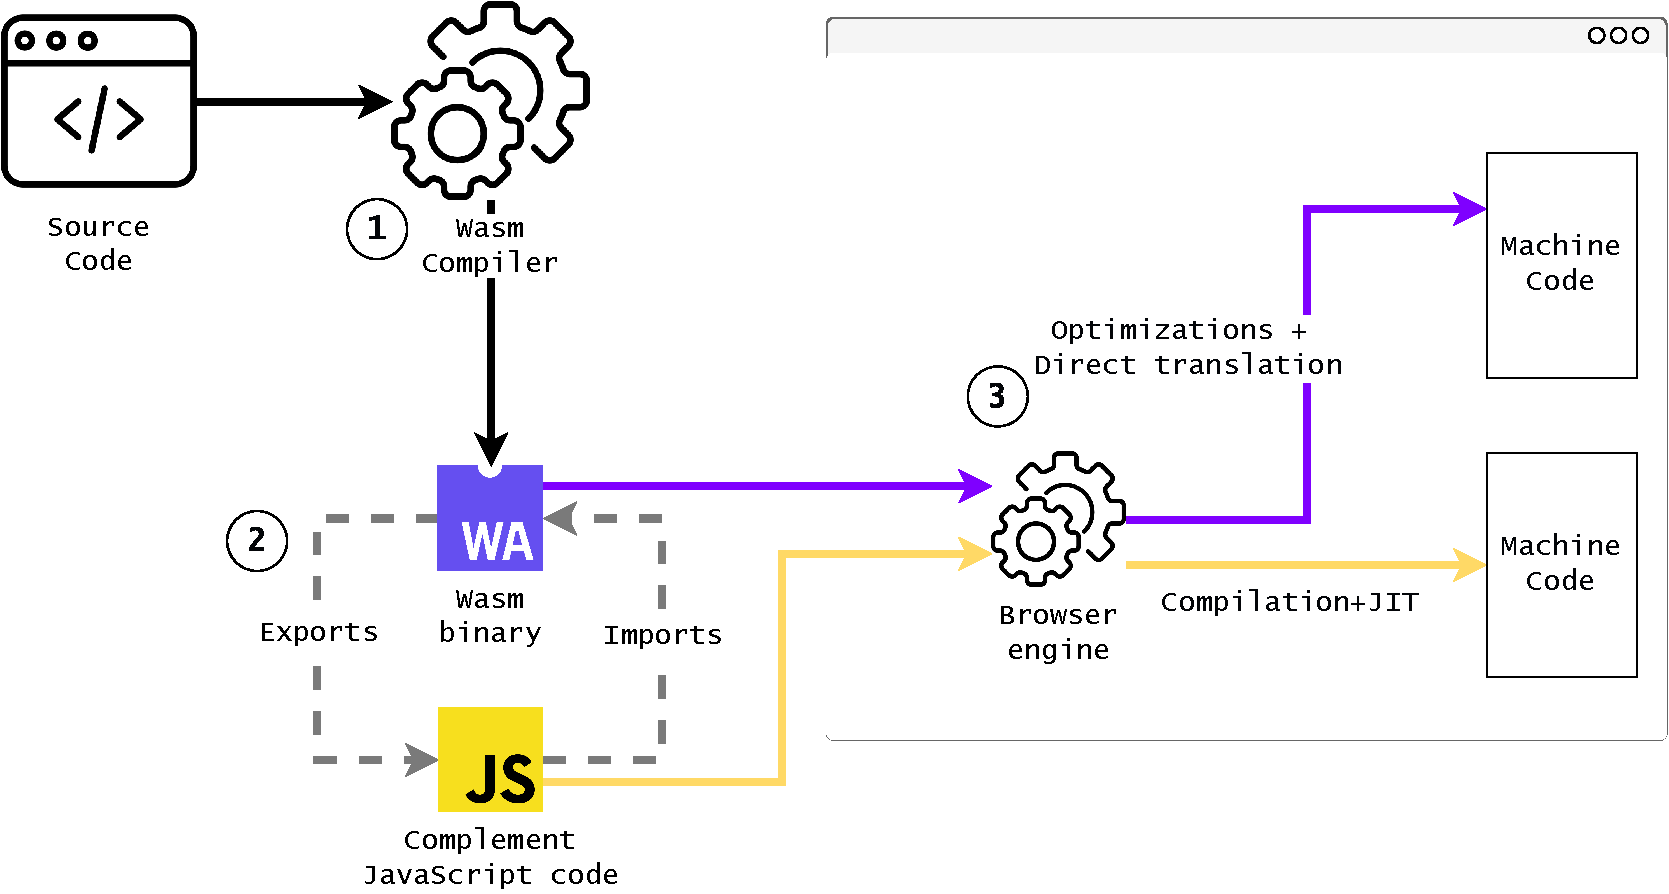
\includegraphics[width=\linewidth]{diagrams/wasm_workflow.pdf}
    \caption{TODO1.}
    \label{diagrams:sota:wasm}
\end{figure}

The Wasm binary might not need external glue code. Thus, depends on the host environment and the binary itself to supply it. This fact encourages the adoption of \wasm further browser engines. For instance, Cloudflare and Fastly adapted their platforms to provide Function as a Service (FaaS) directly with \wasm. In this case the glue code, instead of JavaScript, is provided by any other language stack that the host environment supports.
In 2019, the bytecode alliance team \footnote{\url{https://bytecodealliance.org/}} proposed WebAssembly System Interface (WASI). WASI is the foundation to build Wasm code outside of the browser with a POSIX system interface platform. It standarizes the adoption of \wasm outside web browsers \cite{bryant2020webassembly} in heterogeneous platforms like the Edge or IoT \cite{Narayan2021Swivel,Sledge}. 

% Talk about benchmarks and performance numbers

%Previous studies resulted in performance increasing in terms of bandwidth saving, execution, and process-on-demand spawning \cite{9640153, wen2020wasmachine}. The words of Solomon Hykes \footnote{\url{https://twitter.com/solomonstre/status/1111004913222324225}}, the former CEO of docker, show the impact of WASI: 

%\begin{displayquote}
%\textit{
%    If WASM+WASI existed in 2008, we wouldn't have needed to created Docker. That's how important it is. Webassembly on the server is the future of computing. A standardized system interface was the missing link. Let's hope WASI is up to the task!
%}
%\end{displayquote}

%\todo{How to obtain WebAssembly binaries}

%\todo{Browser workflow}

%\todo{How interpreters work, explain the workflow of V8 as it was validated by the V8 compiler developers}

%\todo{Backend workflow}

%\todo{Add a table with tools and interpreters: V8, SpiderMonkey, wasmtime, wasmer, sledge, warduino }


\subsection*{Instruction Set Architecture}

% General description
\wasm defines its out Instruction Set Architecture (ISA). It is an abstraction close to machine code instructions but agnostic to CPU architectures. Thus, Wasm is platform independent. The ISA of Wasm includes also the necessary components that the binary requires to run in any host engine. These components include the memory model and bytecode instructions.
A Wasm binary has a module as its main component (according to the current roadmap and supported version in all Wasm vendors). A module is composed by 12 \todo{check} types of sections, each of them with an explicit semantic and a specific order inside the module. This makes the compilation to machine code faster. The binary format of Wasm can include custom sections. For example, the work of \todo{Doe} proposed the usage of custom sections to sign binaries for the sake of trusting.

% Example
\begin{code}
    \lstset{language=C,caption={C function that calculates the quantity $2x + x$},label=CExample}
\begin{lstlisting}[style=CStyle]
int f(int x) { 
    return 2 * x + x; 
}

int main(void) { 
    return f(10); 
}
\end{lstlisting}
    
\lstset{
        language=WAT,
        caption={\wasm code  for \autoref{CExample}.},
        style=WATStyle,
        stepnumber=0,
        label=WASMExample}

\begin{lstlisting}
(module
    (type (;0;) (func (param i32) (result i32)))
    (type (;1;) (func (result i32)))
    (func (;0;) (type 0) (param i32) (result i32)
        local.get 0
        local.get 0
        i32.const 2
        i32.mul
        i32.add)
    (func (;1;) (type 1) (result i32)
        i32.const 10
        call 0)
    (export "main" (func 1)))
\end{lstlisting}
\end{code}


% Fast, instructions, fast parsing, compile as it comes

% Portable, unrelated to CPU architectures, some number on size vs JS code

% Self contained loops

% Bound memory, no direct access to the DOM

% Roadmap: threads, SIMD, etc

\todo{Internals of WebAssembly}

\todo{Wasm Semantics: Add a code listing, explain General layout of a binary, Function and signature, Instructions, Control flow, Memory model, Global model, table model}

\todo{Add some sentences from the roadmap}

\todo{Exported function signature allows typing validation before the code is executed}


\subsection*{Wasm security}


\begin{comment}

\todo{Add example...}
\todo{Go slow...}
\todo{Toolchain, explain frontends, general pipeline...}

In this section, we introduce an overview of the motivation for \wasm and its usage. 
\todo{Jumps to fast, avoid !. Sentece 2} Besides, we describe the process to obtain Wasm programs and how this novel technology evolves from being only-browser-based to standalone executions in the backend. Nevertheless, we describe its significant limitations regarding security, that is our main motivation for our research.

\todo{Why Wasm, asm.js, from source to Wasm, mention benchmarks and examples, photoshop, games, etc, data types, memory model, stack modeling, from Wasm to execution, finalize with security, benefits and limitations. Add diagram}
\todo{The need of a virtual machine or a compiler.}
\todo{Why backend, why WASI as an extension not an essential part of Wasm for the browser.}

\todo{Add diagram, for obtaining Wasm and executing them, with references}
% What is Wasm


% How to generate Wasm code
\wasm binaries are obtained from source code like C/C++ or Rust \cite{Hilbig2021AnES}. The \wasm code is further interpreted or compiled ahead of time into machine code by engines such as the browsers. Since version 8, LLVM supports Wasm as a backend opening the door for its vast collection of frontend languages. The LLVM support was encouraged by the seminal work of Zakai \etal with Emscripten.
Emscripten is an open-source tool for compiling C/C++ to the \wasm. It uses LLVM to create Wasm, but it provides support for faster linking to the object files. Instead of all the IR being compiled by LLVM, the object file is prelinked with Wasm in a faster way. 

\subsection*{\wasm for backend execution}



% Why is important to study Wasm
\subsection*{\wasm security and our motivation for diversification}


\wasm is characterized by a robust security model~\cite{WebAssemblySecurity}. It should run inside a sandboxed execution environment that provides protection against common security issues such as data corruption, code injection, and return-oriented programming (ROP). However, WebAssembly is vulnerable under certain conditions, at the execution engine's level \cite{ChromeZero} or the binary itself ~\cite{usenixWasm2020}.
Implementations in both browsers and standalone runtimes~\cite{Narayan2021Swivel} are vulnerable.
This means that if one environment is vulnerable, all the others are vulnerable in the same manner as the same \wasm binary is replicated, turning it into a monoculture problem.


On the other hand, the \wasm environment lacks natural diversity \cite{natural_diversity}. Compared to the work of Harrand \etal \citationneeded, in WebAssembly, one could not use preexisting and different program versions to provide diversification for monoculture solving. In fact, according to the work of Hilbig \etal \cite{Hilbig2021AnES}, the artificial variants created with one of our works contribute to the half of executable and available \wasm binaries in the wild. 


The current limitations on security and the lack of preexisting diversity motivate our work on software diversification as one possible mitigation among the wide range of security countermeasures. 

\end{comment}
